\documentclass[11pt]{article}

% Packages
\usepackage{titlesec} % for customizing section titles
\usepackage{lipsum} % for dummy text
\usepackage{graphicx, subfig} % for including images
\usepackage{float} % for precise image placement with [H] option
\usepackage{biblatex} % for bibliography
\usepackage[a4paper, total={6in, 8in}]{geometry}
\usepackage{hyperref}

% Title setup
\title{\textbf{Autonomous Agents Report}}
\author{Christos Dimas \\ AM : 2021030183}
\date{April 17, 2024 \\~\\~\\~\\}
% Section title formatting
\titleformat{\section}
{\normalfont\Large\bfseries}{\thesection}{1em}{}

% Begin document

\begin{document}

\begin{figure}[t]
    \centering
    
\includegraphics[width=0.5\textwidth]{Images/tuc_image.png}
\end{figure}

% Title
\maketitle

\begin{center}
    \textbf{Project's topic}\\~\\
    Agent Training to recognise Invasive Ductal Carcinoma (IDC), the most common subtype of all breast cancers, given breast histopathology images, with the use of Deep Learning
\end{center}

\newpage
% Table of Contents
\tableofcontents

\newpage

% Sections
\section{Introduction}
\begin{minipage}{\textwidth}
Nowadays, medicine has made huge steps forward, there are still many health problems that are not completely solved. One of those and probably the most major one is the disease of cancer. This was the reason why I decided to make a project to predict breast cancer, a form of cancer that causes the death of 670,000 women annually. \\~\\
So to solve the problem I decided to build a Convolutional Neural Network (CNN) in Python and train it properly on a database with histopathology images. The agent is used to process those images and then predict the state of the patients health, more specifically if they are positive or negative in the disease of breast cancer. 
\end{minipage}

\section{Data Management}
\subsection{Visualization}
% Example of including an image
The first step to complete the project was to choose and understand the dataset that it needs to train the model. First of all, the dataset was fully labeled, which helps to train the model the right way and also to visualize the given data. \\~\\
To visualize the data, it was split in 2 sets, the positive and the negative ones, and then with the use of Python modules there was created at first a data frame (pandas module) and then a histogram (plotly.express module), to see how the dataset is distributed, and a matrix of images and their labels (numpy, keras.preprocessing and matplotlib.pyplot modules).
\begin{figure}[H]
    \centering
    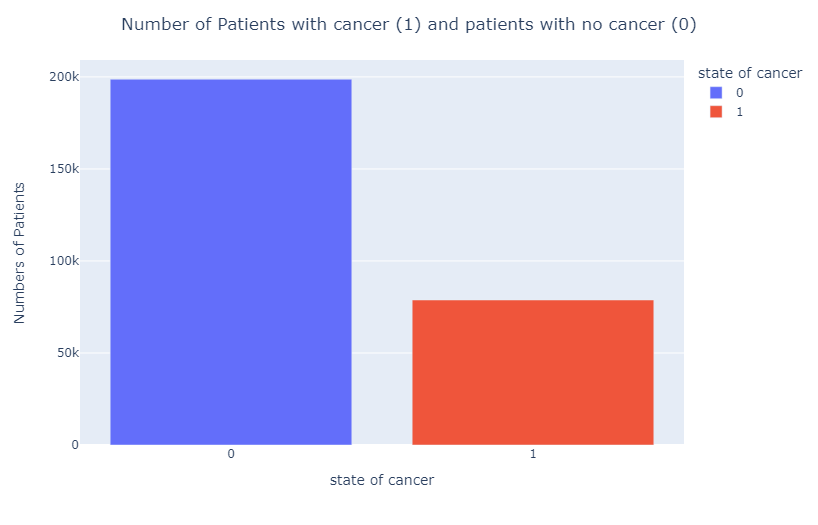
\includegraphics[width=0.7\textwidth]{Images/Histogram.png}
    \caption{Data distribution}
    \label{fig:Figure1}
\end{figure}
\begin{figure}[H]
    \centering
    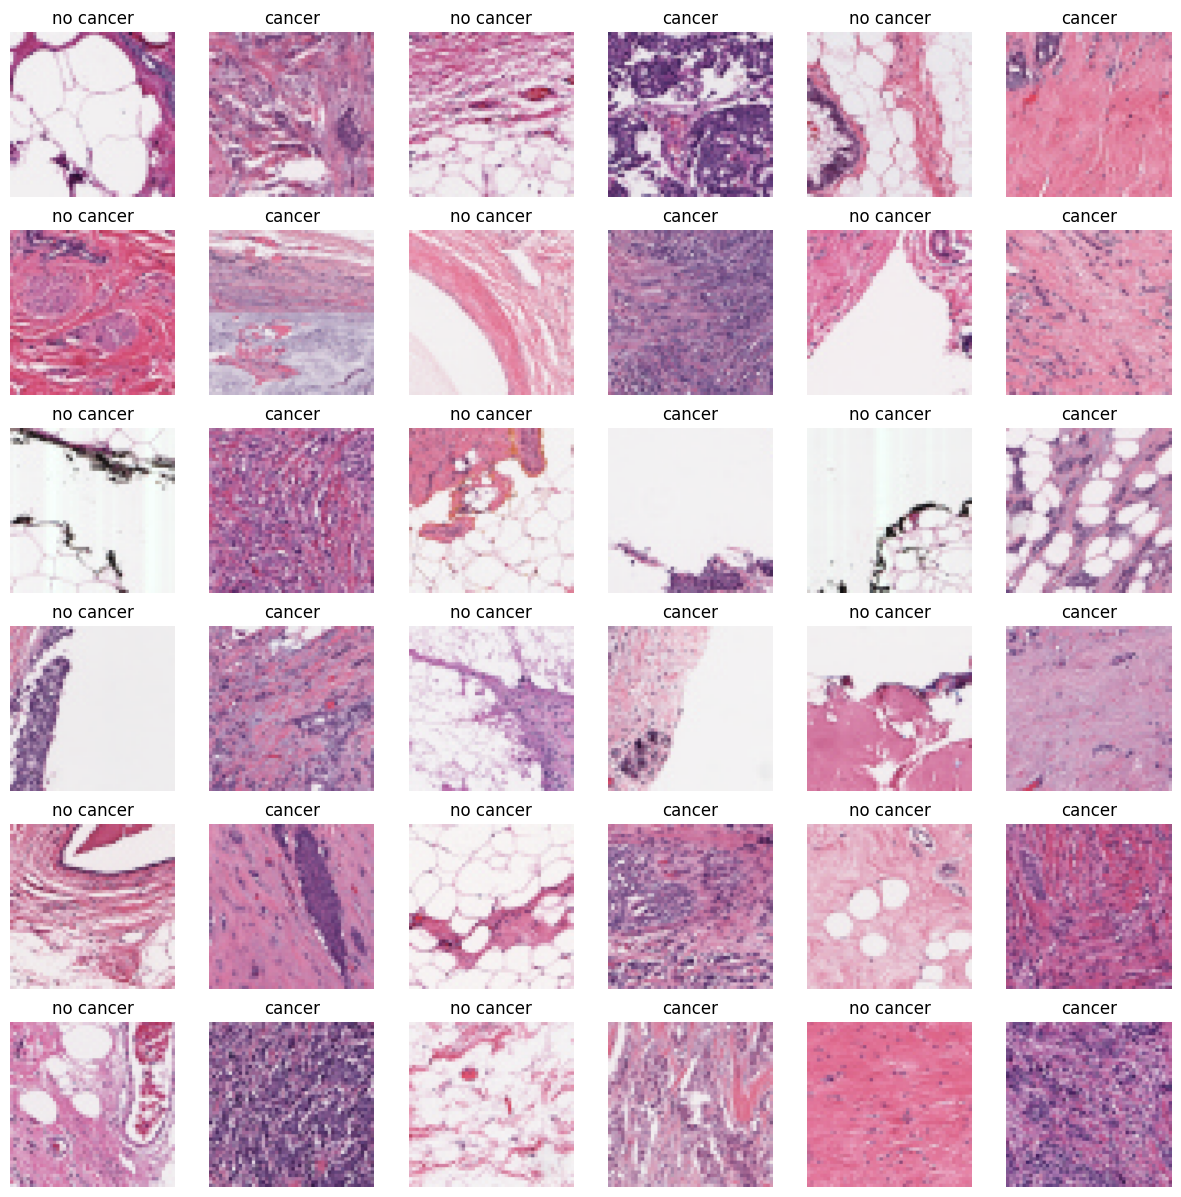
\includegraphics[width=0.5\textwidth]{Images/DataVisualization.png}
    \caption{Data Visualization}
    \label{fig:example}
\end{figure}


\subsection{Preprocessing}

Before the training procedure the data that was split before on two sets, non cancer and cancer, are getting resized so the training is more reliable and then they are put to new lists with their labels. After that the two lists are concatenated and split back, with the criterion of being an image or label into two different arrays (X, Y). At the final step the data was encoded using the one-hot encoding, to represent categorical variables as numerical values that is quite beneficial in the current project. Finally, the parameters of the training are ready and the only thing left is to separate the labeled data in to training and testing set, used for validation and testing (validation was avoided because of the small dataset). The percentage of split was chosen after many trials and the most efficient was the following :
\begin{figure}[H]
    \centering
    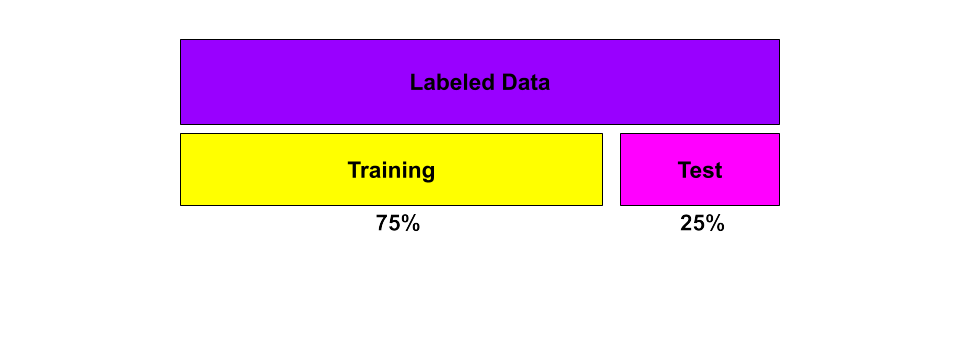
\includegraphics[width=0.6\textwidth]{Images/Data Split.png}
    \caption{Data Split}
    \label{fig:example}
\end{figure}

\section{Agent}
\subsection{Modules used}
To build the network, the Keras API was used. Keras is a deep learning API written in Python, running on the TensorFlow machine learning platform.\\~\\
The network model was based on data processing through the Deep Learning process. Algorithms are based on processing and collection
data using multiple neurons, where each of them receives information, processes it and output a result. Specifically multiply each of their inputs with the corresponding synaptic weight and calculate the total sum of the products. This sum is fed as an argument to one
activation function, where each node implements internally. The value that the function takes for the said argument is also the output of the neuron for the current inputs and weights. \\~\\
In this implementation, the Sequential model, provided by Keras, is used and is nothing other than a linear stack of layers, where each layer consists of neurons. Neurons from different layers are connected to each other, and with appropriate weights, depending on the type of layer used.\\~\\
For image processing, which is required to solve the problem, convolutional layers and computational layers (Dense Layers, Pooling Layers, Flatten Layers) are used. The particular neurons process the information at each level and pass it on to the next. More specifically:
\begin{itemize}
\item Convolutional layers in each unit, neuron takes an image as an input, apply a filter(or kernel) to it and output the results to neurons of the next layer. Overall, each layer apply a series of several filters where they map onto the image and extract details from it. Such details may be edge detection, bright and dark areas, information where they help the network learn and operate on patterns. 
\item Dense layers help to change the dimension of the input information, so that the model to be able to easily define the relationship between the data values on which it operates. These layers are usually used at the end of the model and take as an input, the output of Cl. Depending on the information, the output of each layer get the corresponding weights.
\item Pooling layers are applied after the convolutional layer. The main purpose of pooling is to reduce the size of feature maps, which in turn make computation faster because the number of training parameters is reduced.
\item Flatten layers are used to convert all the resultant 2-Dimensional arrays from pooled feature maps into a single long continuous linear vector. The flattened matrix is fed as an input to the fully connected layer to classify the image.
\end{itemize}
The following Python modules where used in order to implement the things mentioned before:
\begin{itemize}
  \item from sklearn.model\_selection import train\_test\_split
  \item from keras.utils import to\_categorical
  \item import tensorflow 
\end{itemize}
\subsection{Optimizer}
In order to train the models apart from their building blocks, it is necessary to define the process that the network is going to learn throughout the training. However, because of the large number of parameters, choosing the right weights for the model and in a relatively quick time can be a quite challenging task for the builder of the network. \\~\\
For this reason, the use of an optimization algorithm (optimizer) was decided, so that it modifies the characteristics of the neural network, such as the weights and the learning rate, leading to an immediate reduction of total loss and improving accuracy. The optimizer used in this case is Adam with one relatively low learning rate, set as 0.001.
\subsection{Model}
For the creation of the model, a specific architecture was chosen. That came up after many trials in the model and constantly monitoring the results of the training and evaluation processes.\\~\\
The previously mentioned architecture consists : 
\begin{itemize}
  \item At first, a Convolutional Layer is being put into the architecture that has the size of the input (50,50) with 32 filters. After that the data was passed to a max\_pooling layer, so the size can be reduced (25,25) and their characteristics get more obvious.
  \item After that we repeat the previous step for 3 more times. Firstly, the input shape is (25,25) but with 64 filters, with the same procedure as before using max\_pooling and reducing the size to (12,12). The second time the input shape is (12,12), the filters are 128 and max\_pooling reduces the size once more on to (5,5). The final time the input shape of the Convolutional Layer is (5,5) and reduced to a (2,2) after max\_pooling, keeping the filters the same as before.
  \item In the end, we add a Flatten Layer to transform the 2-dimensional array we receive after the previous layers to a vector so we can simplify the classification process. After having converted the data into a one-dimensional sequence, in order to reduce the effect of overfitting on the data with which the model is trained (not to learn specific patterns). The last stage of the network consists of two Dense Layers. The first sized 128 to reduce the data and the second, sized 2, to output the two probabilities of the objects it was trained on.
\end{itemize}
Additionally, each Convolutional Layer and the first Dense use the Rectified Linear Unit (ReLU) activation function, to activate the corresponding nodes and calculate the corresponding weights. Function's type is ReLU(x) = max(0,x), with x being the inputs and is returned when it is positive, otherwise 0 is returned. The last Dense Layer uses softmax as activitation function in order to output a probability distribution over the two possible classes and allow the CNN to make more accurate predictions.\\~\\
Furthermore, each layer has its strides set to 2. As a result the filter will move two pixels to the right at each step instead of one. This means the filter would be applied fewer times, and the resulting output (often referred to as a feature map) would be smaller. Also, same padding is used to keep the output size equal to the input size after convolution.\\~\\
The model analytically and graphicly:
\begin{figure}[H]
    \centering
    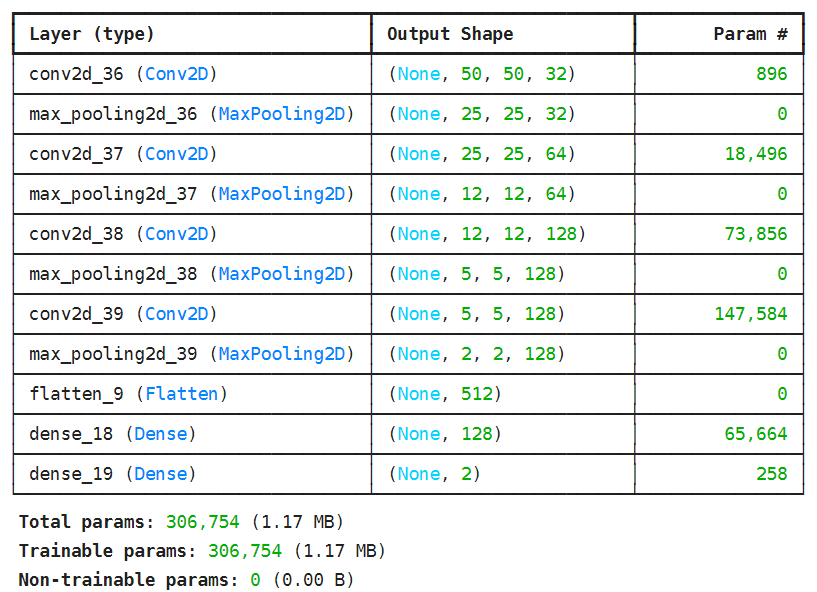
\includegraphics[width=0.8\textwidth]{Images/Screenshot 2024-04-15 184102.png}
    \caption{CNN model matrix}
    \label{fig:example}
\end{figure}
\begin{figure}[H]
    \centering
    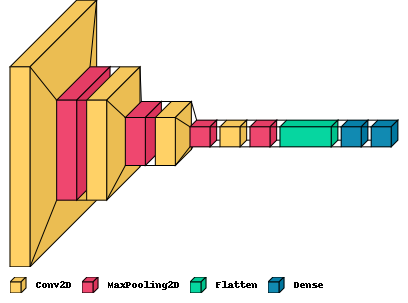
\includegraphics[width=0.8\textwidth]{Images/download.png}
    \caption{CNN model 3D Visualization}
    \label{fig:example}
\end{figure}

\section{Agent Training}
\subsection{Training process}
The training process was highly demanding concerning the computational resources and the size of the dataset (277,524 images) so it was decided to execute the procedure using cloud resources, specifically in a Kaggle notebook so the dataset can be accessed with ease. In order for the network to be trained properly the arrays X and Y where "fed" to the neurons in batches and for a specific number of times to complete many cycles of training and get more reliable weight values therefore better training results.\\~\\ More specifically the batch size was set to 75 as long as there where available resources to use and reduce the mistakes. The number of training cycles, which are called epochs, was set to 25 because while monitoring the results they where stabilized to certain values. Also, a part of the dataset was used to validate the dataset and continuously adjust the weights to achieve better and more accurate results, by preventing overfitting.\\~\\~\\~\\~\\~\\
Console's output in each epoch : 
\begin{figure}[H]
  \centering
  \subfloat[]{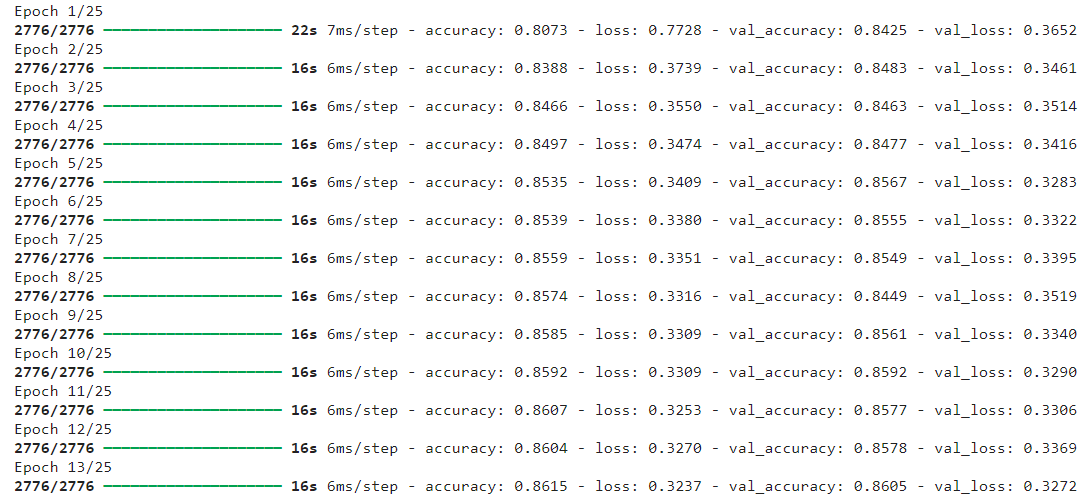
\includegraphics[width=.49\linewidth]{Images/epoch1.png}}\hfill
  \subfloat[] {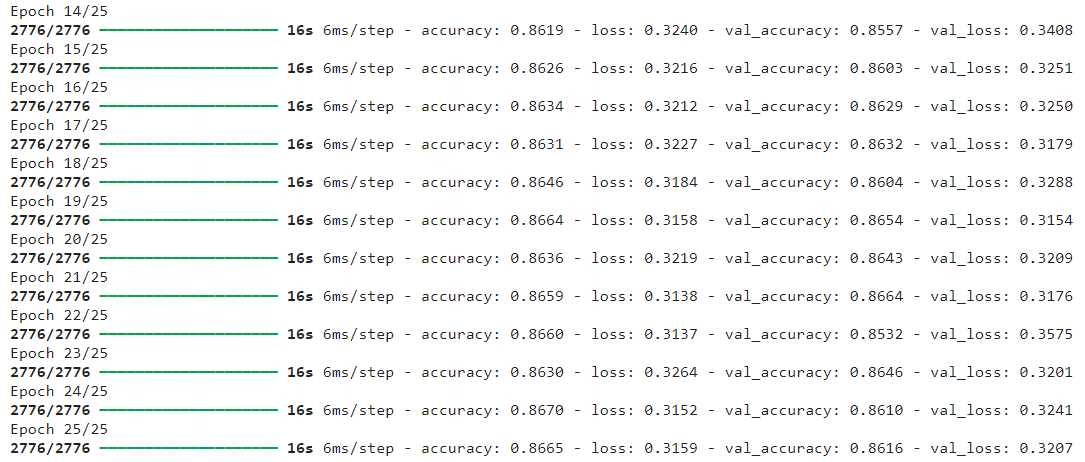
\includegraphics[width=.51\linewidth]{Images/epoch2.png}}
  \caption{Training Process}
\end{figure}
The model's result for it's accuracy and loss in the training process:
\begin{figure}[H]
  \centering
  \subfloat[Accuracy Plot]{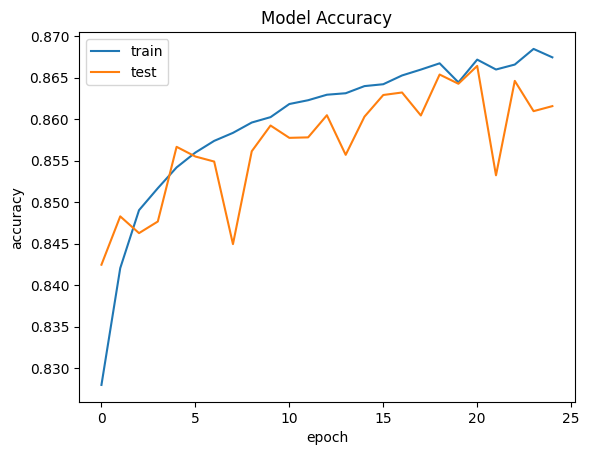
\includegraphics[width=.49\linewidth]{Images/Accuracy.png}}\hfill
  \subfloat[Loss Plot] {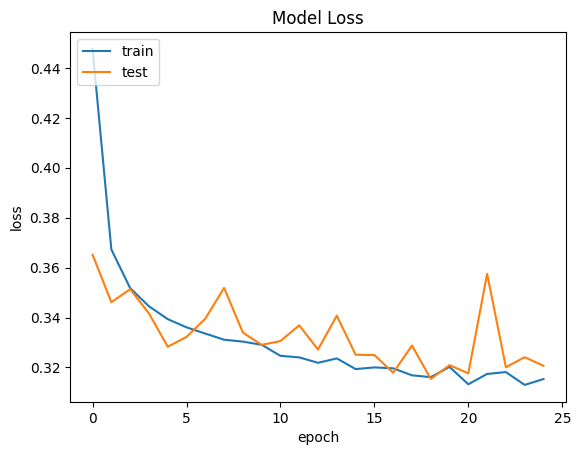
\includegraphics[width=.49\linewidth]{Images/Loss.png}}
  \caption{Training Overview}
\end{figure}

As it seems the average values of the validation and training are pretty close and in a satisfactory level, when taking into account that we deal with image recognition and in order to achieve better results it is needed a more analytic dataset and further training time.
\newpage
\section{Agent Testing}
In order to test the created agent the data that where splitted for training are used and to present the result a Confusion Matrix was created. In that way it can be seen how many of the true lables the model was able to predict after the training and the results are the following :
\begin{figure}[H]
    \centering
    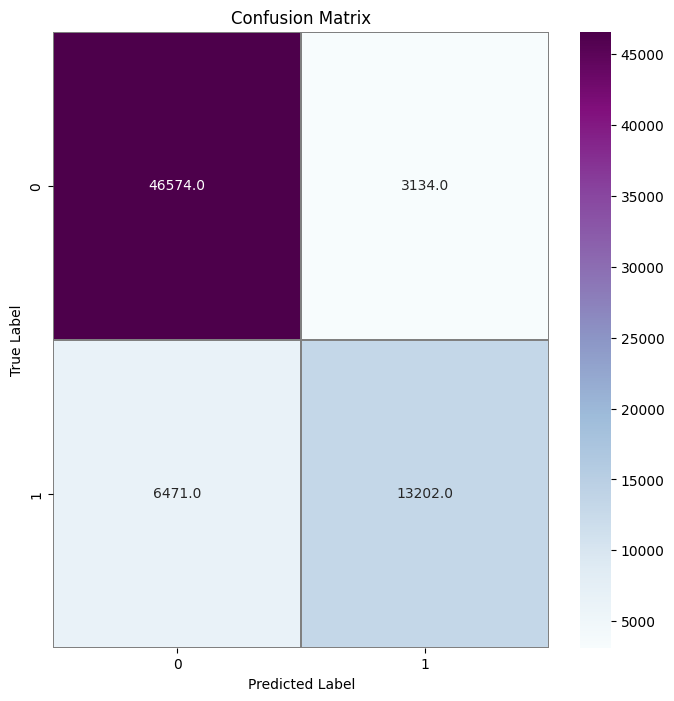
\includegraphics[width=0.7\textwidth]{Images/confusion.png}
    \caption{Data Split}
    \label{fig:example}
\end{figure}
In that way it is observed that works pretty well in general terms since the accuracy of the prediction was at the 84,9\%, a percentage near to the one that was achieved in training. However, even thought in the negative cases the model predicts succesfully the 93.7\% of the cases as negative, in the positive cases it performs significantly lower at 67.1\%, but that is probably due to the unbalanced dataset, that as we can see in \autoref{fig:Figure1} it has much more negative cases than positive (198,738 IDC negative and 78,786 IDC positive).

\section{Breast Cancer Detection}
\subsection{App}
To solve the initial problem it was created a small app that takes an image from the test dataset and print its label. After that the model predicts the value of the particular image and prints the comparison between the true label and the predicted one. This app can easily be expanded further in a next stage of development to take as input new histopathology images. 
The test image:
\begin{figure}[H]
    \centering
    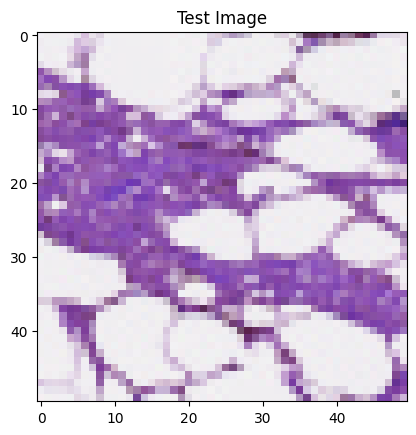
\includegraphics[width=0.6\textwidth]{Images/test_image.png}
    \caption{Test Image}
    \label{fig:example}
\end{figure}
The particular results for the image above:
\begin{figure}[H]
    \centering
    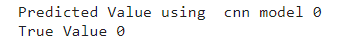
\includegraphics[width=0.6\textwidth]{Images/results.png}
    \caption{Results}
    \label{fig:example}
\end{figure}
\subsection{Problems faced}
The main problem that I faced during the creation of the project was the lack of computer resources that was solved with the help of cloud services. An other problem was that the dataset was not fully appropriate because of the inequality of the samples in our cases and its small size for this kind of use.
\subsection{Conclusion}
In conclusion, creating the project we managed to recognise Invasive Ductal Carcinoma, the most common subtype of all breast cancers, taking as input breast histopathology images. The agent can predict the result with 84.9\% accuracy and even thought it is not in a satisfactory level of accuracy, when thinking about the ethical part of creating a tool that can have appliance in medicine, it was a great way to become familiar with the concept of deep learning and the use of neural networks.

\section{References}
\begin{itemize}
  \item Dataset :  \href{https://www.kaggle.com/datasets/paultimothymooney/breast-histopathology-images/data}{Images}
  \item Cource's book :
  \href{https://www.google.com/search?q=τεχνητή+νοημοσύνη+μια+σύγχρονη+προσέγγιση+4h+ekdosh&client=opera&hs=n79&sca_esv=00980f6df5fed681&prmd=visnbz&sxsrf=ACQVn0_dZwrzQ3-RWJTv6ZM17dYHbBfDiw:1713282338477&source=lnms&sa=X&ved=2ahUKEwiH-byJiseFAxWHhP0HHbRJC24Q0pQJegQIAxAC&biw=1482&bih=706&dpr=1.25}{Artificial Intelligence : One modern approach, 4th American version}
  \item Deep Learning Fundamentals : \href{https://deeplizard.com/learn/playlist/PLZbbT5o_s2xq7LwI2y8_QtvuXZedL6tQU}{Course}
  \item Ideas for the implementation : \href{https://wisdomml.in/breast-cancer-prediction-using-machine-learning/}{Link}
  \item Knowledge for Keras API : \href{https://www.tensorflow.org/guide/keras}{Link}
\end{itemize}
% References (if needed)
\newpage
\printbibliography

\end{document}
